\documentclass[12pt]{article}
\usepackage{../../../lecture_notes}
\usepackage{../../../math}
\usepackage{../../../uark_colors}
\hypersetup{
  colorlinks = true,
  allcolors = ozark_mountains,
  breaklinks = true,
  bookmarksopen = true
}

\begin{document}
\begin{center}
  {\Huge\bf Midterm - Fall 2024}
  
  \smallskip
  {\large\it  ECON 5783 — University of Arkansas}
\end{center}

\medskip
\begin{enumerate}
%   \item Say a researcher wants to model the conditional expectation of wages given gender, college degree, and age. What should the author do if they want to `flexibly' model the conditional expectation function? 

  \item A researcher wants to test the folk-wisdom that playing classical music for children benefits their future academic achievement. The researcher surveys parents and records their high-school GPA ($Y_i$) and whether or not they listened to classical music ($D_i$) as a child.
  \begin{enumerate}
    \item In this context, describe in words what the potential outcomes, $Y_i(0)$ and $Y_i(1)$, are.
    
    \item Do you think the difference-in-means estimator would be biased in this context? If so, which direction do you the treatment effect estimate is biased?
    
    \item Why might a table of summary statistics consisting of sample means of observables, broken down by $D_i = 0$ and $D_i = 1$, be useful in this setting?
  \end{enumerate}

  \medskip
  \item Say you believe the conditional independence assumption $(Y_i(1), Y_i(0)) \Perp D_i \ \vert \ X_i$ holds. 
  \begin{enumerate}
    \item In words, describe what the steps you would take to use a nearest-neighbor matching-based estimator of the treatment effect
    
    \item Say a reader had some concern that overlap would hold in the given application. Why might a balance table be useful for this reader? 
  \end{enumerate}
  
  \medskip
  \item The simplest treatment effect estimator in a setting where you believe the conditional independence assumption is to difference-in-means estimation for individuals with the same values of $X_i = x$ (e.g. separate estiamtes for male and females). The overall treatment effect is formed as a weighted average of the estimates $\widehat{\text{CATE}}(x)$.
  \begin{enumerate}
    \item Describe why the curse of dimensionality makes this infeasible in many settings.
  \end{enumerate}
\end{enumerate}


\bigskip
\noindent
For the following questions refer to Figure \ref{fig:huh_reif_2021}. 
These are two figures from the paper ``Teenage Driving, Mortality, and Risky Behaviors'' in AER: Insights. 
The authors want to study teenage driving on risky behavior and mortality. 
They use a state's minimum driving-age as the cutoff and age as a running variable. 
Those under the minimum age law can not drive and those above can. 

\medskip
\begin{enumerate}
  \setcounter{enumi}{3}
  \item Figure \ref{fig:huh_reif_2021}(a) presents their main results (separately for male and female drivers). 
  They argue that the jump in deaths by motor vehicle accidents is from the driver's ability to drive. 
  What assumptions do we need to make for this RD to identify the causal effect? 
  I am not looking for the `generic' assumption here; I want you to describe the assumption in the context of the research question.
 
  \medskip
  \item The authors present figure \ref{fig:huh_reif_2021}(b) that shows the jump in deaths from `Any Cause' is the same magnitude as the jump \emph{just} from motor vehicle accidents. 
  Do you think this figure helps strengthen their causal claim? Why or why not? 
\end{enumerate}

\medskip
\begin{figure}[htb!]
  \caption{Results from Huh and Reif (2021, AER Insights)}
  \label{fig:huh_reif_2021}
  \begin{center}
    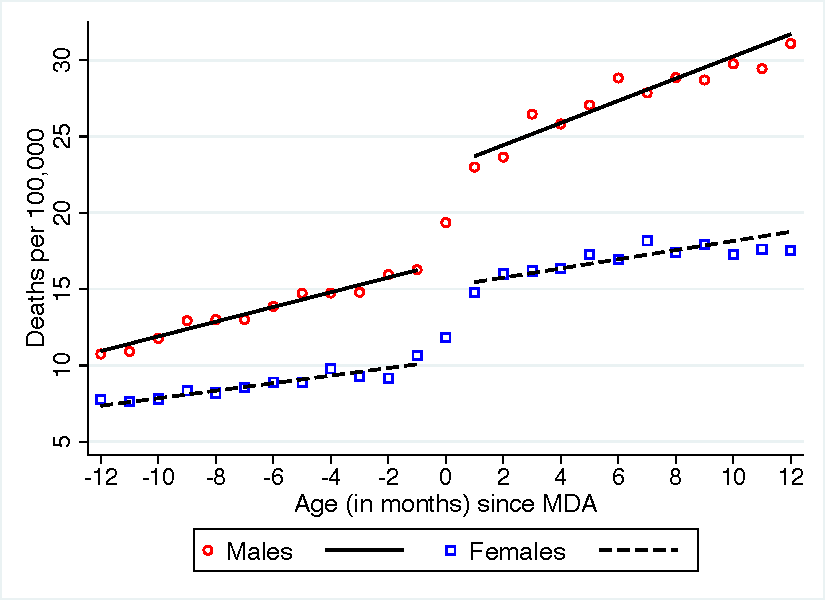
\includegraphics[width = 0.6\textwidth]{rd_mva_male_female.pdf}
    \subcaption{Deaths by Motor Vehicle Accidents}
  \end{center}

  \begin{center}
    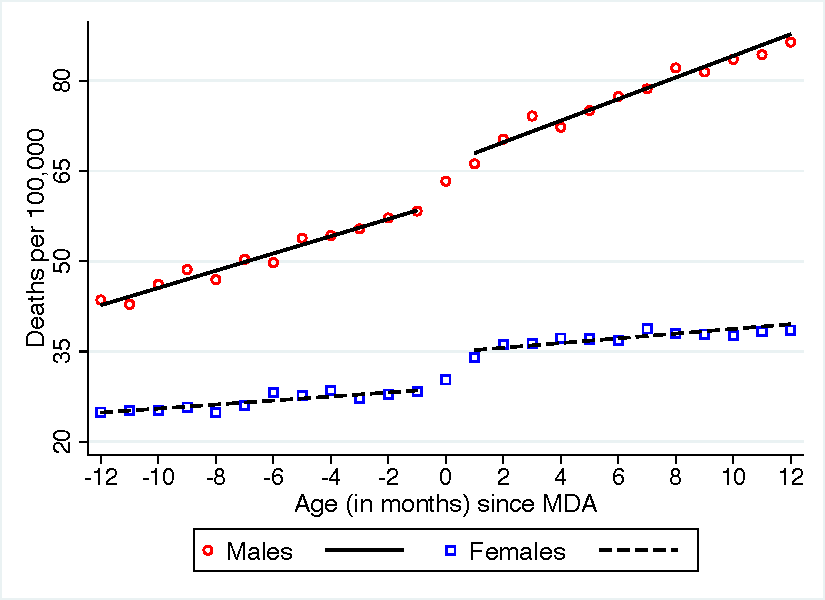
\includegraphics[width = 0.6\textwidth]{rd_any_male_female.pdf}
    \subcaption{Deaths by Any Cause}
  \end{center}
\end{figure}

\end{document}
